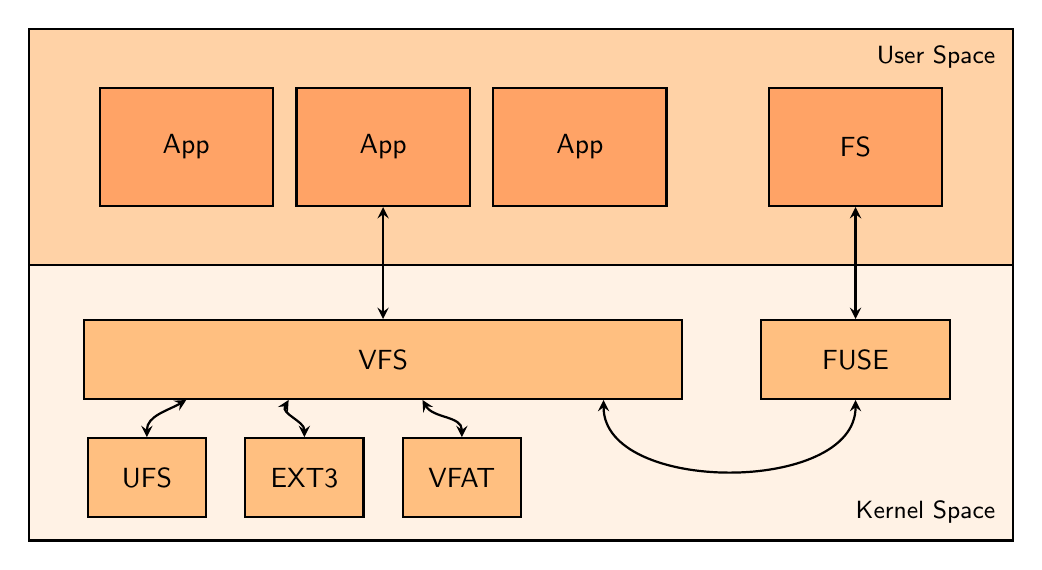
\begin{tikzpicture}[
    % Estilos de colores y cajas para clavarlo a tu imagen
    userbg/.style={fill=orange!35, thick, draw=black},
    kernelbg/.style={fill=orange!10, thick, draw=black},
    appbox/.style={draw=black, thick, fill=orange!80!red!60, minimum width=2.2cm, minimum height=1.5cm, font=\sffamily},
    kernelbox/.style={draw=black, thick, fill=orange!50, minimum height=1cm, font=\sffamily},
    arrow/.style={<->, thick, >=stealth}
]

% 1. Fondos (Cajas grandes de área)
\draw[kernelbg] (0, 0) rectangle (12.5, 3.5);
\draw[userbg] (0, 3.5) rectangle (12.5, 6.5);

% 2. Textos de las áreas (Modified label for User Space)
\node[anchor=north east, font=\sffamily\small] at (12.4, 6.4) {User Space}; % Changed to English, same position

% 3. Cajas del Área de Usuario (Naranja oscuro)
\node[appbox] (app1) at (2, 5) {App};
\node[appbox] (app2) at (4.5, 5) {App};
\node[appbox] (app3) at (7, 5) {App};
\node[appbox] (fs)   at (10.5, 5) {FS};

% 4. Cajas del Área de Kernel (Naranja claro)
\node[kernelbox, minimum width=7.6cm] (vfs) at (4.5, 2.3) {VFS};
\node[kernelbox, minimum width=2.4cm] (fuse) at (10.5, 2.3) {FUSE};

\node[kernelbox, minimum width=1.5cm] (ufs)  at (1.5, 0.8) {UFS};
\node[kernelbox, minimum width=1.5cm] (ext3) at (3.5, 0.8) {EXT3};
\node[kernelbox, minimum width=1.5cm] (vfat) at (5.5, 0.8) {VFAT};

% New English Kernel Space label, tucked neatly into the bottom-right corner *inside* the box
\node[anchor=south east, font=\sffamily\small] at (12.4, 0.1) {Kernel Space}; % Changed to English, new position

% 5. Flechas verticales rectas
\draw[arrow] (app2.south) -- (vfs.north);
\draw[arrow] (fs.south) -- (fuse.north);

% 6. Flechas inferiores curvas hacia VFS
\draw[arrow] (ufs.north) to[out=90, in=210] ([xshift=-2.5cm]vfs.south);
\draw[arrow] (ext3.north) to[out=90, in=240] ([xshift=-1.2cm]vfs.south);
\draw[arrow] (vfat.north) to[out=90, in=300] ([xshift=0.5cm]vfs.south);

% 7. Flecha curva larga (de VFS a FUSE)
\draw[arrow] ([xshift=2.8cm]vfs.south) .. controls +(down:1.2) and +(down:1.2) .. (fuse.south);

\end{tikzpicture}